\documentclass[12pt]{article}
\usepackage{geometry}
\geometry{
	left=20mm,
	top=20mm,
}
\usepackage[utf8]{inputenc}
\usepackage[shortlabels]{enumitem}
\usepackage{array}
\usepackage{tabularx}
\usepackage[table]{xcolor}
\setlength{\arrayrulewidth}{1.5pt}
%\usepackage[xcdraw]{xcolor}

\newcolumntype{C}[1]{>{\centering\let\newline\\\arraybackslash\hspace{0pt}}m{#1}}
\usepackage[spanish,es-nodecimaldot]{babel}
 \usepackage{url}
 \usepackage{hyperref}
 \hypersetup{
 	colorlinks=true,
 	linkcolor=blue,
 	filecolor=magenta,      
 	urlcolor=cyan,
 }
 
 \urlstyle{same}
\usepackage[spanish, fixlanguage]{babelbib}
\bibliographystyle{IEEEtran}
\usepackage{graphicx}
\usepackage{booktabs}
\graphicspath{ {./images/} }
\usepackage{amssymb}
\usepackage{amsmath}
\usepackage{subcaption}
\usepackage[linesnumbered]{algorithm2e}
\newcommand\mycommfont[1]{\footnotesize\ttfamily\textcolor{blue}{#1}}
\SetCommentSty{mycommfont}
\usepackage{tikz}
\usetikzlibrary{positioning, fit}
\usetikzlibrary{babel}
\usetikzlibrary{arrows}
\usepackage{titlesec}
\titlespacing*{\section}
{0pt}{5.5ex plus 1ex minus .2ex}{.3ex plus .1ex}
\titlespacing*{\subsection}
{0pt}{5.5ex plus 1ex minus .2ex}{2.3ex plus .1ex}
\title{Tarea 4: Gráficos probabilísticos}
\newcommand{\otoprule}{\midrule[\heavyrulewidth]}
\author{
	Saul Ivan Rivas Vega \\
	\\
	Aprendizaje Automatizado\\
}

\date{\today}

\begin{document}
	\maketitle
	\pagebreak
	\section{Ejercicio 1}
	  \paragraph{} En una planta nuclear hay una alarma que se activa cuando un indicador de temperatura excede un umbral. El indicador mide la temperatura del núcleo. Considera las variables booleanas $A$ (alarma), $D_A$ (alarma defectuosa), $D_I$ (indicador defectuoso) y las variables enteras $I$ (lectura del indicador) y $T$ (temperatura real del núcleo).
	  \begin{itemize}
		\item Dibuja 3 redes bayesianas válidas diferentes que capturen el comportamiento del proceso, entre ellas incluye aquella que capture el mayor número de independencias condicionales con el menor número de arcos. Discute el modelo representado por cada una de las redes.
		\item De las redes dibujadas, escribe sus distribuciones conjuntas en términos de sus probabilidades condicionales.
		\item Asumiendo que las variables enteras $I$ y $T$ pueden tomar un máximo de 100 valores, ¿Cuál sería el número de valores necesarios en cada nodo y el total en cada una de las redes?
	  \end{itemize}
	  \subsection{}
	  \begin{figure}[h!]
	  	\begin{center}
	  		\begin{tikzpicture}[->,>=stealth',shorten >=1pt,auto,node distance=3cm,
	  		thick,main node/.style={circle,draw,font=\sffamily\Large\bfseries}]
	  		
	  		\node[main node] (1) {$T$};
	  		\node[main node] (2) [below left of=1] {$D_I$};
	  		\node[main node] (3) [below of=1] {$I$};
	  		\node[main node] (4) [below of=3] {$A$};
	  		\node[main node] (5) [right of=3] {$D_A$};
	  		
	  		\path[every node/.style={font=\sffamily\small}]
	  		(1) edge node [left] {}(3)
	  		(1) edge node [left] {}(2)
	  		(1) edge node [left] {}(5)
	  		(2) edge node [left] {}(3)
	  		(3) edge node [left] {}(4)
	  		(5) edge node [left] {}(4);
	  		\end{tikzpicture}
	  	\end{center}
	  	\caption{Red 1.}
	  	\label{fig:ej1001}
	  \end{figure}
  En esta red se interpreta que si la temperatura tenga cierto valor, influye en la probabilidad de que tanto el indicador como la alarma sean defectuosos esto es por la intuición de que quizá ambos funcionen perfectamente hasta que la temperatura del núcleo este en valores muy altos. De igual forma la temperatura influye directamente en el valor que este reportando el indicador. El indicador se ve influenciado naturalmente por la probabilidad de que este sea defectuoso. Para que la alarma este activa influye si es defectuosa y también el valor que este reportando el indicador.\\
  Su distribución conjunta en términos de sus probabilidades condicionales es:
\begin{equation}
	P(T,D_I,I,D_A,A)=P(T)P(D_I|T)P(I|D_I,T)P(D_A|T)P(A|I,D_A)
\end{equation}
\begin{table}[h!]
	\centering
	\begin{tabular}{|c|c|c|c|c|c|}
		\hline
		\rowcolor[gray]{.8}
	\multicolumn{6}{|c|}{$P(T)$} \\\hline %
		\rowcolor[gray]{.8}
		0 & 1 & 2 & 3 & $\dots$ & 99\\\hline
		$P(T=0)$ & $P(T=1)$ & $P(T=2)$ & $P(T=3)$ & $\dots$ & $P(T=99)$\\\hline
	\end{tabular}
\caption{Tabla de valores para la variable $\pmb{T}$, son \textbf{100}.}
\label{tab:ej1001}0
\end{table}
\begin{table}[h!]
	\centering
	\begin{tabular}{|c|c|c|}
		\hline
		\rowcolor[gray]{.8}
		$T$&$P(D_I=0|T)$&$P(D_I=1|T)$ \\\hline %
		0 & $P(D_I=0|T=0)$ &$P(D_I=1|T=0)$\\\hline
		1 & $P(D_I=0|T=1)$ &$P(D_I=1|T=1)$\\\hline
		2 & $P(D_I=0|T=2)$ &$P(D_I=1|T=2)$\\\hline
		$\dots$ & $\dots$ &$\dots$\\\hline
		99 & $P(D_I=0|T=99)$ &$P(D_I=1|T=99)$\\\hline
	\end{tabular}
	\caption{Tabla de valores para la variable $\pmb{D_I}$, son \textbf{200} ($D_I\times T=2\times 100$).}
	\label{tab:ej1002}
\end{table}
\begin{table}[h!]
	\centering
	\begin{tabular}{|c|c|c|}
		\hline
		\rowcolor[gray]{.8}
		$T$&$P(D_A=0|T)$&$P(D_A=1|T)$ \\\hline %
		0 & $P(D_A=0|T=0)$ &$P(D_A=1|T=0)$\\\hline
		1 & $P(D_A=0|T=1)$ &$P(D_A=1|T=1)$\\\hline
		2 & $P(D_A=0|T=2)$ &$P(D_A=1|T=2)$\\\hline
		$\dots$ & $\dots$ &$\dots$\\\hline
		99 & $P(D_A=0|T=99)$ &$P(D_A=1|T=99)$\\\hline
	\end{tabular}
	\caption{Tabla de valores para la variable $\pmb{D_A}$, son \textbf{200} ($D_A\times T=2\times 100$).}
	\label{tab:ej1003}
\end{table}
\begin{table}[h!]
	\centering
	\begin{tabular}{|c|c|c|c|c|c|}
		\hline
		\rowcolor[gray]{.8}
		$D_I$&$T$&$P(I=0|T,D_I)$ &$P(I=1|T,D_I)$&$\dots$&$P(I=99|T,D_I)$ \\\hline %
		0 & 0 & $P(I=0|T=0,D_I=0)$ &$P(I=1|T=0,D_I=0)$&$\dots$&$P(I=99|T=0,D_I=0)$\\\hline
		0 & 1 & $P(I=0|T=1,D_I=0)$ &$P(I=1|T=1,D_I=0)$&$\dots$&$P(I=99|T=1,D_I=0)$\\\hline
		0 & 2 & $P(I=0|T=2,D_I=0)$ &$P(I=1|T=2,D_I=0)$&$\dots$&$P(I=99|T=2,D_I=0)$\\\hline
		0 & $\dots$ & $\dots$ &$\dots$&$\dots$&$\dots$\\\hline
		0 & 99 & $P(I=0|T=99,D_I=0)$ &$P(I=1|T=99,D_I=0)$&$\dots$&$P(I=99|T=99,D_I=0)$\\\hline
		1 & 0 & $P(I=0|T=0,D_I=1)$ &$P(I=1|T=0,D_I=1)$&$\dots$&$P(I=99|T=0,D_I=1)$\\\hline
		1 & 1 & $P(I=0|T=1,D_I=1)$ &$P(I=1|T=1,D_I=1)$&$\dots$&$P(I=99|T=1,D_I=1)$\\\hline
		1 & 2 & $P(I=0|T=2,D_I=1)$ &$P(I=1|T=2,D_I=1)$&$\dots$&$P(I=99|T=2,D_I=1)$\\\hline
		1 & $\dots$ & $\dots$ &$\dots$&$\dots$&$\dots$\\\hline
		1 & 99 & $P(I=0|T=99,D_I=1)$ &$P(I=1|T=99,D_I=1)$&$\dots$&$P(I=99|T=99,D_I=1)$\\\hline
	\end{tabular}
	\caption{Tabla de valores para la variable $\pmb{I}$, son \textbf{20000} ($D_I\times T\times I=2\times 100\times 100$).}
	\label{tab:ej1004}
\end{table}
\begin{table}[h!]
	\centering
	\begin{tabular}{|c|c|c|c|}
		\hline
		\rowcolor[gray]{.8}
		$D_A$&$I$&$P(A=0|I,D_A)$&$P(A=1|I,D_A)$ \\\hline %
		0 & 0 & $P(A=0|I=0,D_A=0)$ &$P(A=1|I=0,D_A=0)$\\\hline
		0 & 1 & $P(A=0|I=1,D_A=0)$ &$P(A=1|I=1,D_A=0)$\\\hline
		0 & 2 & $P(A=0|I=2,D_A=0)$ &$P(A=1|I=2,D_A=0)$\\\hline
		0 & $\dots$ & $\dots$ &$\dots$\\\hline
		0 & 99 & $P(A=0|I=99,D_A=0)$ &$P(A=1|I=99,D_A=0)$\\\hline
		1 & 0 & $P(A=0|I=0,D_A=1)$ &$P(A=1|I=0,D_A=1)$\\\hline
		1 & 1 & $P(A=0|I=1,D_A=1)$ &$P(A=1|I=1,D_A=1)$\\\hline
		1 & 2 & $P(A=0|I=2,D_A=1)$ &$P(A=1|I=2,D_A=1)$\\\hline
		1 & $\dots$ & $\dots$ &$\dots$\\\hline
		1 & 99 & $P(A=0|I=99,D_A=1)$ &$P(A=1|I=99,D_A=1)$\\\hline
	\end{tabular}
	\caption{Tabla de valores para la variable $\pmb{A}$, son \textbf{400} ($A\times I\times D_A=2\times 100 \times 2$).}
	\label{tab:ej1005}
\end{table}\pagebreak
\paragraph{} Finalmente tomando en cuenta los valores obtenidos de las 5 tablas obtenemos el total de valores en la red:
\begin{equation}
	100 + 200 + 200 + 20000 + 400 = 20900
\end{equation}
\pagebreak
	  \subsection{}
	  \begin{figure}[h!]
	  	\begin{center}
	  		\begin{tikzpicture}[->,>=stealth',shorten >=1pt,auto,node distance=3cm,
	  		thick,main node/.style={circle,draw,font=\sffamily\Large\bfseries}]
	  		
	  		\node[main node] (1) {$T$};
	  		\node[main node] (2) [below left of=1] {$D_I$};
	  		\node[main node] (3) [below of=1] {$I$};
	  		\node[main node] (4) [below of=3] {$A$};
	  		\node[main node] (5) [right of=3] {$D_A$};
	  		
	  		\path[every node/.style={font=\sffamily\small}]
	  		(1) edge node [left] {}(3)
	  		(1) edge node [left] {}(2)
	  		(2) edge node [left] {}(3)
	  		(3) edge node [left] {}(4)
	  		(5) edge node [left] {}(4);
	  		\end{tikzpicture}
	  	\end{center}
	  	\caption{Red 2.}
	  	\label{fig:ej1002}
	  \end{figure}
  En esta red se interpreta prácticamente lo mismo que en el anterior sin embargo se busca introducir mas independencias condicionales y minimizar los arcos sin interferir demasiado en la intuición de la red original. Aquí la temperatura deja de influir para el evento de que la alarma sea defectuosa. Un ejemplo de independencia condicional que se agrega es $D_I  \perp\!\!\!\perp D_A | I$, porque ahora los caminos de $D_I$ a $D_A$ son: $\{D_I,T,I,A,D_A\}$ y $\{D_I,I,A,D_A\}$ y tienen las tripletas $[\{D_I,T,I\}, \{T,I,A\}, \{I,A,D_A\}]$ y $[\{D_I,I,A\}, \{I,A,D_A\}]$ respectivamente. Y dado $I$ la tripleta del primer camino $\{T,I,A\}$ y la tripleta del segundo camino $\{D_I,I,A\}$ son inactivas ya que ambas son cadenas causales con la variable observada en medio, entonces ningún camino es activo y por lo tanto $D_I$ es condicionalmente independiente de $D_A$ dado $I$.\\
  Su distribución conjunta en términos de sus probabilidades condicionales es:
  \begin{equation}
  P(T,D_I,I,D_A,A)=P(T)P(D_A)P(D_I|T)P(I|D_I,T)P(A|I,D_A)
  \end{equation}
\begin{table}[h!]
	\centering
	\begin{tabular}{|c|c|c|c|c|c|}
		\hline
		\rowcolor[gray]{.8}
		\multicolumn{6}{|c|}{$P(T)$} \\\hline %
		\rowcolor[gray]{.8}
		0 & 1 & 2 & 3 & $\dots$ & 99\\\hline
		$P(T=0)$ & $P(T=1)$ & $P(T=2)$ & $P(T=3)$ & $\dots$ & $P(T=99)$\\\hline
	\end{tabular}
	\caption{Tabla de valores para la variable $\pmb{T}$, son \textbf{100}.}
	\label{tab:ej1006}0
\end{table}
\begin{table}[h!]
	\centering
	\begin{tabular}{|c|c|c|}
		\hline
		\rowcolor[gray]{.8}
		$T$&$P(D_I=0|T)$&$P(D_I=1|T)$ \\\hline %
		0 & $P(D_I=0|T=0)$ &$P(D_I=1|T=0)$\\\hline
		1 & $P(D_I=0|T=1)$ &$P(D_I=1|T=1)$\\\hline
		2 & $P(D_I=0|T=2)$ &$P(D_I=1|T=2)$\\\hline
		$\dots$ & $\dots$ &$\dots$\\\hline
		99 & $P(D_I=0|T=99)$ &$P(D_I=1|T=99)$\\\hline
	\end{tabular}
	\caption{Tabla de valores para la variable $\pmb{D_I}$, son \textbf{200} ($D_I\times T=2\times 100$).}
	\label{tab:ej1007}
\end{table}
\begin{table}[h!]
	\centering
	\begin{tabular}{|c|c|}
		\hline
		\rowcolor[gray]{.8}
		\multicolumn{2}{|c|}{$P(D_A)$} \\\hline %
		\rowcolor[gray]{.8}
		0 & 1 \\\hline
		$P(D_A=0)$ & $P(D_A=1)$\\\hline
	\end{tabular}
	\caption{Tabla de valores para la variable $\pmb{D_A}$, son \textbf{2}.}
	\label{tab:ej1008}
\end{table}
\begin{table}[h!]
	\centering
	\begin{tabular}{|c|c|c|c|c|c|}
		\hline
		\rowcolor[gray]{.8}
		$D_I$&$T$&$P(I=0|T,D_I)$ &$P(I=1|T,D_I)$&$\dots$&$P(I=99|T,D_I)$ \\\hline %
		0 & 0 & $P(I=0|T=0,D_I=0)$ &$P(I=1|T=0,D_I=0)$&$\dots$&$P(I=99|T=0,D_I=0)$\\\hline
		0 & 1 & $P(I=0|T=1,D_I=0)$ &$P(I=1|T=1,D_I=0)$&$\dots$&$P(I=99|T=1,D_I=0)$\\\hline
		0 & 2 & $P(I=0|T=2,D_I=0)$ &$P(I=1|T=2,D_I=0)$&$\dots$&$P(I=99|T=2,D_I=0)$\\\hline
		0 & $\dots$ & $\dots$ &$\dots$&$\dots$&$\dots$\\\hline
		0 & 99 & $P(I=0|T=99,D_I=0)$ &$P(I=1|T=99,D_I=0)$&$\dots$&$P(I=99|T=99,D_I=0)$\\\hline
		1 & 0 & $P(I=0|T=0,D_I=1)$ &$P(I=1|T=0,D_I=1)$&$\dots$&$P(I=99|T=0,D_I=1)$\\\hline
		1 & 1 & $P(I=0|T=1,D_I=1)$ &$P(I=1|T=1,D_I=1)$&$\dots$&$P(I=99|T=1,D_I=1)$\\\hline
		1 & 2 & $P(I=0|T=2,D_I=1)$ &$P(I=1|T=2,D_I=1)$&$\dots$&$P(I=99|T=2,D_I=1)$\\\hline
		1 & $\dots$ & $\dots$ &$\dots$&$\dots$&$\dots$\\\hline
		1 & 99 & $P(I=0|T=99,D_I=1)$ &$P(I=1|T=99,D_I=1)$&$\dots$&$P(I=99|T=99,D_I=1)$\\\hline
	\end{tabular}
	\caption{Tabla de valores para la variable $\pmb{I}$, son \textbf{20000} ($D_I\times T\times I=2\times 100\times 100$).}
	\label{tab:ej1009}
\end{table}
\begin{table}[h!]
	\centering
	\begin{tabular}{|c|c|c|c|}
		\hline
		\rowcolor[gray]{.8}
		$D_A$&$I$&$P(A=0|I,D_A)$&$P(A=1|I,D_A)$ \\\hline %
		0 & 0 & $P(A=0|I=0,D_A=0)$ &$P(A=1|I=0,D_A=0)$\\\hline
		0 & 1 & $P(A=0|I=1,D_A=0)$ &$P(A=1|I=1,D_A=0)$\\\hline
		0 & 2 & $P(A=0|I=2,D_A=0)$ &$P(A=1|I=2,D_A=0)$\\\hline
		0 & $\dots$ & $\dots$ &$\dots$\\\hline
		0 & 99 & $P(A=0|I=99,D_A=0)$ &$P(A=1|I=99,D_A=0)$\\\hline
		1 & 0 & $P(A=0|I=0,D_A=1)$ &$P(A=1|I=0,D_A=1)$\\\hline
		1 & 1 & $P(A=0|I=1,D_A=1)$ &$P(A=1|I=1,D_A=1)$\\\hline
		1 & 2 & $P(A=0|I=2,D_A=1)$ &$P(A=1|I=2,D_A=1)$\\\hline
		1 & $\dots$ & $\dots$ &$\dots$\\\hline
		1 & 99 & $P(A=0|I=99,D_A=1)$ &$P(A=1|I=99,D_A=1)$\\\hline
	\end{tabular}
	\caption{Tabla de valores para la variable $\pmb{A}$, son \textbf{400} ($A\times I\times D_A=2\times 100 \times 2$).}
	\label{tab:ej1010}
\end{table}\pagebreak
\paragraph{} Finalmente tomando en cuenta los valores obtenidos de las 5 tablas obtenemos el total de valores en la red:
\begin{equation}
100 + 200 + 2 + 20000 + 400 = 20702
\end{equation}
\pagebreak
  \subsection{}
  \begin{figure}[h!]
  	\begin{center}
  		\begin{tikzpicture}[->,>=stealth',shorten >=1pt,auto,node distance=3cm,
  		thick,main node/.style={circle,draw,font=\sffamily\Large\bfseries}]
  		
  		\node[main node] (1) {$T$};
  		\node[main node] (2) [below left of=1] {$D_I$};
  		\node[main node] (3) [below of=1] {$I$};
  		\node[main node] (4) [below of=3] {$A$};
  		\node[main node] (5) [right of=3] {$D_A$};
  		
  		\path[every node/.style={font=\sffamily\small}]
  		(1) edge node [left] {}(3)
  		(2) edge node [left] {}(3)
  		(3) edge node [left] {}(4)
  		(5) edge node [left] {}(4);
  		\end{tikzpicture}
  	\end{center}
  	\caption{Red 3.}
  	\label{fig:ej1003}
  \end{figure}
Finalmente para esta tercer red llegamos a una de las posibilidades de la red inicial con menor numero de arcos y mayor numero de independencias condicionales al quitar la influencia de la temperatura en el evento de que el indicador sea defectuoso. Un ejemplo de independencia condicional que se agrega es $T  \perp\!\!\!\perp A | I$, porque ahora el camino de $T$ a $A$ es uno inactivo dado $I$ ya que es una cadena causal con la variable observada en medio, y por ser el único todos los caminos de $T$ a $A$ están inactivos y por lo tanto $T$ es condicionalmente independiente de $A$ dado $I$.\\
Su distribución conjunta en términos de sus probabilidades condicionales es:
\begin{equation}
P(T,D_I,I,D_A,A)=P(T)P(D_A)P(D_I)P(I|D_I,T)P(A|I,D_A)
\end{equation}
\begin{table}[h!]
	\centering
	\begin{tabular}{|c|c|c|c|c|c|}
		\hline
		\rowcolor[gray]{.8}
		\multicolumn{6}{|c|}{$P(T)$} \\\hline %
		\rowcolor[gray]{.8}
		0 & 1 & 2 & 3 & $\dots$ & 99\\\hline
		$P(T=0)$ & $P(T=1)$ & $P(T=2)$ & $P(T=3)$ & $\dots$ & $P(T=99)$\\\hline
	\end{tabular}
	\caption{Tabla de valores para la variable $\pmb{T}$, son \textbf{100}.}
	\label{tab:ej1011}0
\end{table}
\begin{table}[h!]
	\centering
	\begin{tabular}{|c|c|}
		\hline
		\rowcolor[gray]{.8}
		\multicolumn{2}{|c|}{$P(D_I)$} \\\hline %
		\rowcolor[gray]{.8}
		0 & 1 \\\hline
		$P(D_I=0)$ & $P(D_I=1)$\\\hline
	\end{tabular}
	\caption{Tabla de valores para la variable $\pmb{D_I}$, son \textbf{2} ($D_I\times T=2\times 100$).}
	\label{tab:ej1012}
\end{table}
\begin{table}[h!]
	\centering
	\begin{tabular}{|c|c|}
		\hline
		\rowcolor[gray]{.8}
		\multicolumn{2}{|c|}{$P(D_A)$} \\\hline %
		\rowcolor[gray]{.8}
		0 & 1 \\\hline
		$P(D_A=0)$ & $P(D_A=1)$\\\hline
	\end{tabular}
	\caption{Tabla de valores para la variable $\pmb{D_A}$, son \textbf{2}.}
	\label{tab:ej1013}
\end{table}
\begin{table}[h!]
	\centering
	\begin{tabular}{|c|c|c|c|c|c|}
		\hline
		\rowcolor[gray]{.8}
		$D_I$&$T$&$P(I=0|T,D_I)$ &$P(I=1|T,D_I)$&$\dots$&$P(I=99|T,D_I)$ \\\hline %
		0 & 0 & $P(I=0|T=0,D_I=0)$ &$P(I=1|T=0,D_I=0)$&$\dots$&$P(I=99|T=0,D_I=0)$\\\hline
		0 & 1 & $P(I=0|T=1,D_I=0)$ &$P(I=1|T=1,D_I=0)$&$\dots$&$P(I=99|T=1,D_I=0)$\\\hline
		0 & 2 & $P(I=0|T=2,D_I=0)$ &$P(I=1|T=2,D_I=0)$&$\dots$&$P(I=99|T=2,D_I=0)$\\\hline
		0 & $\dots$ & $\dots$ &$\dots$&$\dots$&$\dots$\\\hline
		0 & 99 & $P(I=0|T=99,D_I=0)$ &$P(I=1|T=99,D_I=0)$&$\dots$&$P(I=99|T=99,D_I=0)$\\\hline
		1 & 0 & $P(I=0|T=0,D_I=1)$ &$P(I=1|T=0,D_I=1)$&$\dots$&$P(I=99|T=0,D_I=1)$\\\hline
		1 & 1 & $P(I=0|T=1,D_I=1)$ &$P(I=1|T=1,D_I=1)$&$\dots$&$P(I=99|T=1,D_I=1)$\\\hline
		1 & 2 & $P(I=0|T=2,D_I=1)$ &$P(I=1|T=2,D_I=1)$&$\dots$&$P(I=99|T=2,D_I=1)$\\\hline
		1 & $\dots$ & $\dots$ &$\dots$&$\dots$&$\dots$\\\hline
		1 & 99 & $P(I=0|T=99,D_I=1)$ &$P(I=1|T=99,D_I=1)$&$\dots$&$P(I=99|T=99,D_I=1)$\\\hline
	\end{tabular}
	\caption{Tabla de valores para la variable $\pmb{I}$, son \textbf{20000} ($D_I\times T\times I=2\times 100\times 100$).}
	\label{tab:ej1014}
\end{table}
\begin{table}[h!]
	\centering
	\begin{tabular}{|c|c|c|c|}
		\hline
		\rowcolor[gray]{.8}
		$D_A$&$I$&$P(A=0|I,D_A)$&$P(A=1|I,D_A)$ \\\hline %
		0 & 0 & $P(A=0|I=0,D_A=0)$ &$P(A=1|I=0,D_A=0)$\\\hline
		0 & 1 & $P(A=0|I=1,D_A=0)$ &$P(A=1|I=1,D_A=0)$\\\hline
		0 & 2 & $P(A=0|I=2,D_A=0)$ &$P(A=1|I=2,D_A=0)$\\\hline
		0 & $\dots$ & $\dots$ &$\dots$\\\hline
		0 & 99 & $P(A=0|I=99,D_A=0)$ &$P(A=1|I=99,D_A=0)$\\\hline
		1 & 0 & $P(A=0|I=0,D_A=1)$ &$P(A=1|I=0,D_A=1)$\\\hline
		1 & 1 & $P(A=0|I=1,D_A=1)$ &$P(A=1|I=1,D_A=1)$\\\hline
		1 & 2 & $P(A=0|I=2,D_A=1)$ &$P(A=1|I=2,D_A=1)$\\\hline
		1 & $\dots$ & $\dots$ &$\dots$\\\hline
		1 & 99 & $P(A=0|I=99,D_A=1)$ &$P(A=1|I=99,D_A=1)$\\\hline
	\end{tabular}
	\caption{Tabla de valores para la variable $\pmb{A}$, son \textbf{400} ($A\times I\times D_A=2\times 100 \times 2$).}
	\label{tab:ej1015}
\end{table}\pagebreak
\paragraph{} Finalmente tomando en cuenta los valores obtenidos de las 5 tablas obtenemos el total de valores en la red:
\begin{equation}
100 + 2 + 2 + 20000 + 400 = 20504
\end{equation}
\pagebreak
	\section{Ejercicio 2}	 
	  \begin{figure}[h!]
	  	\centering
	  	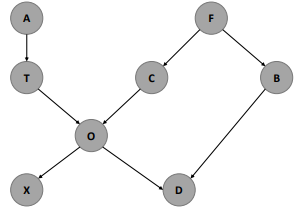
\includegraphics[width=.4\linewidth]{excercise2f}
	  	\caption{Modelo gráfico de diagnóstico de enfermedades de pulmón.}
	  	\label{fig1}
	  \end{figure}
	A una clínica le concierne el diagnóstico de enfermedades de pulmón. Como se puede ver en el modelo de la Figura~\ref{fig1}, una visita a Asia ($A$) hace que la probabilidad de tener tuberculosis ($T$) aumente. Los nodos en la gráfica tienen el siguiente significado:	 
	\begin{figure}[h!]
		\centering
		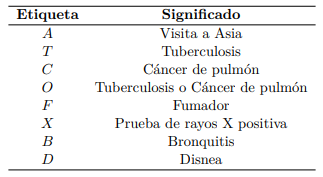
\includegraphics[width=.4\linewidth]{excercise2t}
		\label{table1}
	\end{figure}
Di si las siguientes relaciones de independencia condicional son verdaderas o falsas y explica por qué:
\subsection{$T  \perp\!\!\!\perp F | D$}
De $T$ a $F$ existen 2 caminos de nodos:
\begin{enumerate}
	\item $\{T, O, C, F\}$
	\item $\{T, O, D, B, F\}$
\end{enumerate}
En el Camino 1 existen las siguientes tripletas $[\{T,O,C\},\{O,C,F\}]$, la tripleta $\{T,O,C\}$ esta activa ya que es un efecto común donde uno de los descendientes es la variable observada (en este caso nuestra variable observada $D$ es descendiente de $O$).
La otra tripleta $\{O,C,F\}$ es una cadena causal pero ninguna de sus variables es observada, así decimos que esta activa. Como las 2 tripletas del camino 1 fueron activas, el camino 1 es activo. \\
Como hay al menos un camino activo entre $T$ y $F$ dado $D$ decimos que no se garantiza la independencia condicional y por lo tanto es \textbf{falso} afirmar que $T  \perp\!\!\!\perp F | D$ solo con los datos de la gráfica.
\subsection{$C  \perp\!\!\!\perp B | F$}
De $C$ a $B$ existen 2 caminos de nodos:
\begin{enumerate}
	\item $\{C, F, B\}$
	\item $\{C, O, D, B\}$
\end{enumerate}
En el Camino 1 solo existe la tripleta $\{C,F,B\}$, la cual es inactiva ya que es una causa común donde la variable de en medio $F$ si es observada. Como no todas las tripletas del camino 1 fueron activas decimos que el camino es inactivo.
En el Camino 2 existen las siguientes tripletas $[\{C,O,D\},\{O,D,B\}]$, la tripleta $\{C,O,D\}$ esta activa ya que es una cadena causal donde ninguna variable es observada.
La otra tripleta $\{O,D,B\}$ es un efecto común pero ninguna de sus variables es observada, así decimos que es inactiva. Como no todas las tripletas del camino 1 fueron activas decimos que el camino es inactivo.\\
Finalmente como no hay un solo camino activo entre $C$ y $B$ dado $F$ se garantiza la independencia condicional y por lo tanto es \textbf{verdadero} afirmar que $C  \perp\!\!\!\perp B | F$ solo con los datos de la gráfica.
\subsection{$A  \perp\!\!\!\perp F | C$}
De $A$ a $F$ existen 2 caminos de nodos:
\begin{enumerate}
	\item $\{A, T, O, D, B, F\}$
	\item $\{A, T, O, C, F\}$
\end{enumerate}
En el Camino 1 existen las siguientes tripletas $[\{A,T,O\},\{O,D,B\},\{D,B,F\}]$. La tripleta $\{O,D,B\}$ esta inactiva ya que es un efecto común donde ninguna variable es observada. Como no todas las tripletas del camino 1 son activas decimos que el camino es inactivo.\\
En el Camino 2 existen las siguientes tripletas $[\{A,T,O\},\{O,C,F\}]$. La tripleta $\{O,C,F\}$ esta inactiva ya que es una cadena causal donde la variable de en medio $C$ es observada. Como no todas las tripletas del camino 2 son activas decimos que el camino es inactivo.\\
Finalmente como no hay un solo camino activo entre $A$ y $F$ dado $C$ se garantiza la independencia condicional y por lo tanto es \textbf{verdadero} afirmar que $A  \perp\!\!\!\perp F | C$ solo con los datos de la gráfica.
\subsection{$A  \perp\!\!\!\perp F | C,D$}
De $A$ a $F$ existen 2 caminos de nodos:
\begin{enumerate}
	\item $\{A, T, O, D, B, F\}$
	\item $\{A, T, O, C, F\}$
\end{enumerate}
En el Camino 1 existen las siguientes tripletas $[\{A,T,O\},\{O,D,B\},\{D,B,F\}]$. La tripleta $\{A,T,O\}$ es activa ya que es una cadena causal donde ninguna variable es observada. La tripleta $\{T,O,D\}$ es activa ya que es una cadena causal donde ninguna variable es observada. La tripleta $\{O,D,B\}$ es activa ya que es un efecto común donde la variable de en medio $D$ es observada. La tripleta $\{D,B,F\}$ es activa ya que es una cadena causal que a pesar de que $D$ es observada, esta no es la variable de en medio, en este caso la variable de en medio es $B$ y no es observada. Como todas las tripletas del camino 1 son activas decimos que el camino es activo.\\
Como hay al menos un camino activo entre $A$ y $F$ dado $C,D$ decimos que no se garantiza la independencia condicional y por lo tanto es \textbf{falso} afirmar que $A  \perp\!\!\!\perp F | C,D$ solo con los datos de la gráfica.
\section{Ejercicio 3}
Imagina una clínica que ayuda a pacientes con ébola en un área afectada por el virus. La red de la Figura~\ref{fig2} intenta capturar la dinámica por la cual las personas que sufren los síntomas pueden llegar a esta clínica y ver a un especialista. Existe la posibilidad de que alguien con ébola ($E=\text{verdadero}$) muestre síntomas, por ejemplo sangrado ($S=\text{verdadero}$), fiebre ($F=\text{verdadero}$) y visite la clínica ($V=\text{verdadero}$). El sangrado incrementa el riesgo de complicaciones ($C=\text{verdadero}$) y la persona puede ser llevada a ver un doctor especialista ($D=\text{verdadero}$).
\begin{figure}[h!]
	\centering
	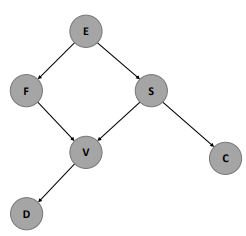
\includegraphics[width=.35\linewidth]{excercise3f}
	\caption{Modelo gráfico de detección de ébola.}
	\label{fig2}
\end{figure}
\pagebreak
\begin{itemize}
	\item $P(E=\text{verdadero})=0.01$
	\item $P(F=\text{verdadero}|E=\text{verdadero})=0.6$
	\item $P(F=\text{verdadero}|E=\text{falso})=0.1$
	\item $P(S=\text{verdadero}|E=\text{verdadero})=0.8$
	\item $P(S=\text{verdadero}|E=\text{falso})=0.05$
	\item $P(V=\text{verdadero}|F=\text{verdadero},S=\text{verdadero})=0.8$
	\item $P(V=\text{verdadero}|F=\text{verdadero},S=\text{falso})=0.5$
	\item $P(V=\text{verdadero}|F=\text{falso},S=\text{verdadero})=0.7$
	\item $P(V=\text{verdadero}|F=\text{falso},S=\text{falso})=0.0$
	\item $P(C=\text{verdadero}|S=\text{verdadero})=0.75$
	\item $P(C=\text{verdadero}|S=\text{falso})=0.1$
	\item $P(D=\text{verdadero}|V=\text{verdadero})=0.6$
	\item $P(D=\text{verdadero}|V=\text{falso})=0.0$
\end{itemize}
Con estas probabilidades y el modelo gráfico de la Figura~\ref{fig2}, realiza lo siguiente:
\subsection{a)} Escribe la distribución conjunta de la red bayesiana en función de las probabilidades condicionales.
\begin{equation}
	P(E,F,S,V,C,D)=P(E)P(F|E)P(S|E)P(V|F,S)P(C|S)P(D|V)
\end{equation}
\subsection{b)} Si un paciente es llevado al doctor ($D=\text{verdadero}$), usando un paquete de software calcula la probabilidad de que no tenga ébola  ($P(E=\text{falso}|D=\text{verdadero})$).\\
En la siguiente liga se encuentra un notebook en Colab describiendo el proceso:\\
\url{https://colab.research.google.com/drive/1BlZamlzMlFqEgX02bqvozlM1_Kb2VQ2D?usp=sharing}\\
El resultado es:
\begin{equation}
P(E=\text{falso}|D=\text{verdadero})=0.9248
\end{equation}
\subsection{c)} Convierte a la red bayesiana en un modelo gráfico no dirigido (campo aleatorio de Markov) y dibújalo. Captura tantas relaciones de independencia condicional como sea posible.
 \begin{figure}[h!]
	\begin{center}
		\begin{tikzpicture}[-,>=stealth',shorten >=1pt,auto,node distance=3cm,
		thick,main node/.style={circle,draw,font=\sffamily\Large\bfseries}]
		
		\node[main node] (1) {$E$};
		\node[main node] (2) [below left of=1] {$F$};
		\node[main node] (3) [below right of=1] {$S$};
		\node[main node] (4) [below left of=3] {$V$};
		\node[main node] (5) [below right of=3] {$C$};
		\node[main node] (6) [below left of=4] {$D$};
		
		\path[every node/.style={font=\sffamily\small}]
		(1) edge node [left] {}(2)
		(1) edge node [left] {}(3)
		(2) edge node [left] {}(4)
		(2) edge node [left] {}(3)
		(3) edge node [left] {}(4)
		(3) edge node [left] {}(5)
		(4) edge node [left] {}(6);
		\end{tikzpicture}
	\end{center}
	\caption{Modelo gráfico no dirigido (Campo aleatorio de Markov).}
	\label{fig:ej2001}
\end{figure}
\subsubsection{Algunas independencias condicionales para el Campo aleatorio de Markov de la figura ~\ref{fig:ej2001}}
Si observamos $S$ y retiramos a $S$ junto con todas sus aristas quedamos con:\\
 \begin{figure}[h!]
	\begin{center}
		\begin{tikzpicture}[-,>=stealth',shorten >=1pt,auto,node distance=3cm,
		thick,main node/.style={circle,draw,font=\sffamily\Large\bfseries}]
		
		\node[main node] (1) {$E$};
		\node[main node] (2) [below left of=1] {$F$};
		\node[main node] (4) [below left of=3] {$V$};
		\node[main node] (5) [below right of=3] {$C$};
		\node[main node] (6) [below left of=4] {$D$};
		
		\path[every node/.style={font=\sffamily\small}]
		(1) edge node [left] {}(2)
		(2) edge node [left] {}(4)
		(4) edge node [left] {}(6);
		\end{tikzpicture}
	\end{center}
	\caption{Campo aleatorio de Markov observando a $S$.}
	\label{fig:ej2002}
\end{figure}\\
Observando a $S$ obteniendo a la figura \ref{fig:ej2002}, $C$ se desconectó de $E$, $F$, $V$ y $D$, por lo que obtenemos las siguientes independencias condicionales:
\begin{itemize}
	\item $E  \perp\!\!\!\perp C | S$
	\item $F  \perp\!\!\!\perp C | S$
	\item $V  \perp\!\!\!\perp C | S$
	\item $D  \perp\!\!\!\perp C | S$
\end{itemize}
Si observamos $V$ y retiramos a $V$ junto con todas sus aristas quedamos con:\\
 \begin{figure}[h!]
	\begin{center}
		\begin{tikzpicture}[-,>=stealth',shorten >=1pt,auto,node distance=3cm,
		thick,main node/.style={circle,draw,font=\sffamily\Large\bfseries}]
		
		\node[main node] (1) {$E$};
		\node[main node] (2) [below left of=1] {$F$};
		\node[main node] (3) [below right of=1] {$S$};
		\node[main node] (5) [below right of=3] {$C$};
		\node[main node] (6) [below left of=4] {$D$};
		
		\path[every node/.style={font=\sffamily\small}]
		(1) edge node [left] {}(2)
		(1) edge node [left] {}(3)
		(2) edge node [left] {}(3)
		(3) edge node [left] {}(5);
		\end{tikzpicture}
	\end{center}
	\caption{Campo aleatorio de Markov observando a $V$.}
	\label{fig:ej2003}
\end{figure}\\
Observando a $V$ obteniendo a la figura \ref{fig:ej2003}, $D$ se desconectó de $E$, $F$, $S$ y $C$, por lo que obtenemos las siguientes independencias condicionales:\\

\begin{itemize}
	\item $E  \perp\!\!\!\perp D | V$
	\item $F  \perp\!\!\!\perp D | V$
	\item $S  \perp\!\!\!\perp D | V$
	\item $C  \perp\!\!\!\perp D | V$
\end{itemize}
\pagebreak
Si observamos a $F$ y a $S$, retirándolos junto con todas sus aristas quedamos con:\\
\begin{figure}[h!]
	\begin{center}
		\begin{tikzpicture}[-,>=stealth',shorten >=1pt,auto,node distance=3cm,
		thick,main node/.style={circle,draw,font=\sffamily\Large\bfseries}]
		
		\node[main node] (1) {$E$};
		\node[main node] (4) [below left of=3] {$V$};
		\node[main node] (5) [below right of=3] {$C$};
		\node[main node] (6) [below left of=4] {$D$};
		
		\path[every node/.style={font=\sffamily\small}]
		(4) edge node [left] {}(6);
		\end{tikzpicture}
	\end{center}
	\caption{Campo aleatorio de Markov observando a $F$ y $S$.}
	\label{fig:ej2004}
\end{figure}\\
Observando a $F$ y $S$ obteniendo a la figura \ref{fig:ej2004}, $E$ se desconectó de $D$, $V$ y $C$. A su vez se desconectó $C$ de $V$ y $D$, por lo que obtenemos las siguientes independencias condicionales:
\begin{itemize}
	\item $C  \perp\!\!\!\perp E | F,S$
	\item $D  \perp\!\!\!\perp E | F,S$
	\item $V  \perp\!\!\!\perp E | F,S$
	\item $D  \perp\!\!\!\perp C | F,S$
	\item $V  \perp\!\!\!\perp C | F,S$
\end{itemize}
\subsection{d)} Debido a una campaña de concientización de la salud, las personas son alentadas a visitar la clínica en caso de que tengan fiebre. Esto incrementa la cantidad de visitas de personas con fiebre sin importar el estado de cualquier otra variable.
\subsubsection{} ¿Qué probabilidades condicionales en la red se modifican debido a este cambio y en qué sentido?
\begin{itemize}
	\item $P(V=\text{verdadero}|F=\text{verdadero},S)$ aumenta.
	\item $P(V=\text{falso}|F=\text{verdadero},S)$ disminuye.
	\item $P(V=\text{verdadero}|F=\text{falso},S=\text{verdadero})$ disminuye.
\end{itemize}
\subsubsection{} Describe cualquier efecto que esto tenga en la proporción de personas con complicaciones que visiten la clínica. Menciona exactamente qué probabilidades condicionales usaste para llegar a tu conclusión.\\

Como la probabilidad condicional para que el paciente presente complicaciones es:\\ $P(C=\text{verdadero}|S)$\\
Esta se ve afectada por la proporción de personas con sangrado ya que $P(C=\text{verdadero}|S=\text{verdadero})$ es mucho mayor a $P(C=\text{verdadero}|S=\text{falso})$.
Ahora la campaña de concientización directamente afecta las visitas a la clínica con personas con fiebre es decir:\\ $P(V=\text{verdadero}|F=\text{verdadero},S)$\\
La cual aumenta. Sin embargo como no importa el estado de las demás variables significa que pueden llegar mas pacientes que presenten tanto como fiebre como sangrado, es decir:\\
$P(V=\text{verdadero}|F=\text{verdadero},S=\text{verdadero})$\\
Como no se especifica la proporción con la que llegarán pacientes con fiebre y sangrado o sin sangrado, no podemos suponer que habrá un efecto significativo en la proporción de personas con complicaciones.\\
De existir un efecto se requeriría por ejemplo que la campaña estuviera dirigida a personas con Fiebre pero sin sangrado, esto haría que la presencia de complicaciones estuviera en mayor proporción con:\\
$P(C=\text{verdadero}|S=\text{falso})$\\
El cual es bastante bajo.\\
En el caso contrario donde la campaña estuviera dirigida a personas con Fiebre pero con sangrado, esto haría que la presencia de complicaciones estuviera en mayor proporción con:\\
$P(C=\text{verdadero}|S=\text{verdadero})$\\
El cual es mayor.\\
\subsection{e)} Asume que alguien que no tiene fiebre va al doctor, ¿qué relación de independencia condicional existe en la distribución que no puede ser descubierta a través del grafo solamente?
 \subsection{Opcional} Calcula $P(V|E=\text{verdadero})$ usando el método de eliminación de variables, describiendo de forma detallada el procedimiento que seguiste (2 puntos extras).\\
 Del grafo y las probabilidades dadas, podemos obtener las tablas de valores para cada nodo:\\
 \begin{table}[h!]
 	\centering
 	\begin{tabular}{|c|c|}
 		\hline
 		\rowcolor[gray]{.8}
 		\multicolumn{2}{|c|}{$P(E)$}  \\\hline %
 		$P(E=\text{verdadero})$ & $0.01$\\\hline
 		$P(E=\text{falso})$ & $0.99$\\\hline
 	\end{tabular}
 	\caption{Tabla de valores para la variable $\pmb{E}$, son \textbf{2}.}
 	\label{tab:ej3001}
 \end{table}
\begin{table}[h!]
	\centering
	\begin{tabular}{|c|c|c|}
		\hline
		\rowcolor[gray]{.8}
		$E$&$P(F=\text{verdadero}|E)$&$P(F=\text{falso}|E)$ \\\hline %
		verdadero & $0.6$ &$0.4$\\\hline
		falso & $0.1$ &$0.9$\\\hline
	\end{tabular}
	\caption{Tabla de valores para la variable $\pmb{F}$, son \textbf{4} ($E\times F=2\times 2$).}
	\label{tab:ej3002}
\end{table}
\begin{table}[h!]
	\centering
	\begin{tabular}{|c|c|c|}
		\hline
		\rowcolor[gray]{.8}
		$E$&$P(S=\text{verdadero}|E)$&$P(S=\text{falso}|E)$ \\\hline %
		verdadero & $0.8$ &$0.2$\\\hline
		falso & $0.05$ &$0.95$\\\hline
	\end{tabular}
	\caption{Tabla de valores para la variable $\pmb{S}$, son \textbf{4} ($E\times S=2\times 2$).}
	\label{tab:ej3003}
\end{table}
 \begin{table}[h!]
 	\centering
 	\begin{tabular}{|c|c|c|c|}
 		\hline
 		\rowcolor[gray]{.8}
 		$F$&$S$&$P(V=\text{verdadero}|F,S)$&$P(V=\text{falso}|F,S)$ \\\hline %
 		verdadero & verdadero & $0.8$ &$0.2$\\\hline
 		verdadero & falso & $0.5$ &$0.5$\\\hline
 		falso & verdadero & $0.7$ &$0.3$\\\hline
 		falso & falso & $0.0$ &$1.0$\\\hline
 	\end{tabular}
 	\caption{Tabla de valores para la variable $\pmb{V}$, son \textbf{8} ($F\times S\times V=2\times 2 \times 2$).}
 	\label{tab:ej3004}
 \end{table}
\begin{table}[h!]
	\centering
	\begin{tabular}{|c|c|c|}
		\hline
		\rowcolor[gray]{.8}
		$S$&$P(C=\text{verdadero}|S)$&$P(C=\text{falso}|S)$ \\\hline %
		verdadero & $0.75$ &$0.25$\\\hline
		falso & $0.1$ &$0.9$\\\hline
	\end{tabular}
	\caption{Tabla de valores para la variable $\pmb{C}$, son \textbf{4} ($S\times C=2\times 2$).}
	\label{tab:ej3005}
\end{table}
\begin{table}[h!]
	\centering
	\begin{tabular}{|c|c|c|}
		\hline
		\rowcolor[gray]{.8}
		$V$&$P(D=\text{verdadero}|V)$&$P(D=\text{falso}|V)$ \\\hline %
		verdadero & $0.6$ &$0.4$\\\hline
		falso & $0.0$ &$1.0$\\\hline
	\end{tabular}
	\caption{Tabla de valores para la variable $\pmb{D}$, son \textbf{4} ($V\times D=2\times 2$).}
	\label{tab:ej3006}
\end{table}
\paragraph{} Del inciso a) Obtenemos la distribución Conjunta de toda la red de la cual partimos.
\begin{equation}
\begin{split}
P(E,F,S,V,C,D)&=P(E)P(F|E)P(S|E)P(V|F,S)P(C|S)P(D|V)\\
& \text{Marginalizamos las variables ocultas($F$,$S$,$C$,$D$)}\\
P(V,E=\text{verdadero})&=\\
\sum_{f}\sum_{s}\sum_{c}\sum_{d}[&P(E=\text{verdadero})P(f|E=\text{verdadero})P(s|E=\text{verdadero})P(V|f,s)P(c|s)P(d|V)]\\
& \text{Redistribuimos}\\
P(V,E=\text{verdadero})&=\\
P(E=\text{verdadero})[\sum_{f}&\sum_{s}[P(f|E=\text{verdadero})P(s|E=\text{verdadero})P(V|f,s)\sum_{c}[P(c|s)]\sum_{d}[P(d|V)]]]\\
\end{split}
\end{equation}\\
\paragraph{Eliminamos a $D$}
\begin{equation}
\begin{split}
P(V,E=\text{verdadero})&=\\
P(E=\text{verdadero})[\sum_{f}&\sum_{s}[P(f|E=\text{verdadero})P(s|E=\text{verdadero})P(V|f,s)\sum_{c}[P(c|s)]\sum_{d}[P(d|V)]]]\\
\mathcal{F}_d(V)=& \sum_{d}[P(d|V)]\\
\end{split}
\end{equation}\\
\begin{table}[h!]
	\centering
	\begin{tabular}{|c|c|}
		\hline
		\rowcolor[gray]{.8}
		$V$&$\mathcal{F}_d(V)$ \\\hline %
		verdadero & $0.6+0.4=1.0$\\\hline
		falso & $0.0 + 1.0 = 1.0$\\\hline
	\end{tabular}
	\caption{Tabla de valores para $\mathcal{F}_d(V)$.}
	\label{tab:ej3007}
\end{table}
\begin{equation}
\begin{split}
P(V,E=\text{verdadero})&=\\
P(E=\text{verdadero})[\sum_{f}&\sum_{s}[P(f|E=\text{verdadero})P(s|E=\text{verdadero})P(V|f,s)\sum_{c}[P(c|s)]\mathcal{F}_d(V)]]\\
\end{split}
\end{equation}\\
\paragraph{Eliminamos a $C$}
\begin{equation}
\begin{split}
P(V,E=\text{verdadero})&=\\
P(E=\text{verdadero})[\sum_{f}&\sum_{s}[P(f|E=\text{verdadero})P(s|E=\text{verdadero})P(V|f,s)\sum_{c}[P(c|s)]\mathcal{F}_d(V)]]\\
\mathcal{F}_c(s)=& \sum_{c}[P(c|s)]\\
\end{split}
\end{equation}\\
\begin{table}[h!]
	\centering
	\begin{tabular}{|c|c|}
		\hline
		\rowcolor[gray]{.8}
		$S$&$\mathcal{F}_c(s)$ \\\hline %
		verdadero & $0.75+0.25=1.0$\\\hline
		falso & $0.1 +0.9=1.0$\\\hline
	\end{tabular}
	\caption{Tabla de valores para $\mathcal{F}_c(s)$.}
	\label{tab:ej3008}
\end{table}
\begin{equation}
\begin{split}
P(V,E=\text{verdadero})&=\\
P(E=\text{verdadero})[\sum_{f}[P(f|E=\text{verdadero})&\sum_{s}[P(s|E=\text{verdadero})P(V|f,s)\mathcal{F}_c(s)]\mathcal{F}_d(V)]]\\
\end{split}
\end{equation}\\
\paragraph{Eliminamos a $S$}
\begin{equation}
\begin{split}
P(V,E=\text{verdadero})&=\\
P(E=\text{verdadero})[\sum_{f}[P(f|E=\text{verdadero})&\sum_{s}[P(s|E=\text{verdadero})P(V|f,s)\mathcal{F}_c(s)]\mathcal{F}_d(V)]]\\
\mathcal{F}_s(V,f)=& \sum_{s}[P(s|E=\text{verdadero})P(V|f,s)\mathcal{F}_c(s)]\\
\end{split}
\end{equation}\\
\begin{table}[h!]
	\centering
	\begin{tabular}{|c|c|c|c|}
		\hline
		\rowcolor[gray]{.8}
		$S$&$V$&$F$&$P(s|E=\text{verdadero})P(V|f,s)\mathcal{F}_c(s)$ \\\hline %
		verdadero&verdadero&verdadero & $0.8\times0.8\times1.0=0.64$\\\hline
		verdadero&verdadero&falso & $0.8\times0.7\times1.0=0.56$\\\hline
		verdadero&falso&verdadero & $0.8\times0.2\times1.0=0.16$\\\hline
		verdadero&falso&falso & $0.8\times0.3\times1.0=0.24$\\\hline
		falso&verdadero&verdadero & $0.2\times0.5\times1.0=0.1$\\\hline
		falso&verdadero&falso & $0.2\times0.0\times1.0=0.0$\\\hline
		falso&falso&verdadero & $0.2\times0.5\times1.0=0.1$\\\hline
		falso&falso&falso & $0.2\times1.0\times1.0=0.2$\\\hline
	\end{tabular}
	\caption{Tabla de valores para construir $\mathcal{F}_s(V,f)$.}
	\label{tab:ej3009}
\end{table}
\begin{table}[h!]
	\centering
	\begin{tabular}{|c|c|c|}
		\hline
		\rowcolor[gray]{.8}
		$V$&$F$&$\mathcal{F}_s(V,f)$ \\\hline %
		verdadero&verdadero & $0.64 + 0.1 = 0.74$\\\hline
		verdadero&falso & $0.56 + 0.0 = 0.56$\\\hline
		falso&verdadero & $0.16 + 0.1 = 0.26$\\\hline
		falso&falso & $0.24 + 0.2 = 0.44$\\\hline
	\end{tabular}
	\caption{Tabla de valores para $\mathcal{F}_s(V,f)$.}
	\label{tab:ej3010}
\end{table}
\begin{equation}
\begin{split}
P(V,E=\text{verdadero})&=\\
P(E=\text{verdadero})[\sum_{f}[P(f|E=\text{verdadero})&\mathcal{F}_s(V,f)]\mathcal{F}_d(V)]\\
\end{split}
\end{equation}\\
\paragraph{Eliminamos a $F$}
\begin{equation}
\begin{split}
P(V,E=\text{verdadero})&=P(E=\text{verdadero})[\sum_{f}[P(f|E=\text{verdadero})\mathcal{F}_s(V,f)]\mathcal{F}_d(V)]\\
\mathcal{F}_f(V)=& \sum_{f}[P(f|E=\text{verdadero})\mathcal{F}_s(V,f)]\\
\end{split}
\end{equation}\\
\begin{table}[h!]
	\centering
	\begin{tabular}{|c|c|c|}
		\hline
		\rowcolor[gray]{.8}
		$F$&$V$&$P(f|E=\text{verdadero})\mathcal{F}_s(V,f)$ \\\hline %
		verdadero&verdadero & $0.6\times0.74=0.444$\\\hline
		verdadero&falso & $0.6\times0.26=0.156$\\\hline
		falso&verdadero & $0.4\times0.56=0.224$\\\hline
		falso&falso & $0.4\times0.44=0.176$\\\hline
	\end{tabular}
	\caption{Tabla de valores para construir $\mathcal{F}_f(V)$.}
	\label{tab:ej3011}
\end{table}
\begin{table}[h!]
	\centering
	\begin{tabular}{|c|c|}
		\hline
		\rowcolor[gray]{.8}
		$V$&$\mathcal{F}_f(V)$ \\\hline %
		verdadero & $0.444+0.224=0.668$\\\hline
		falso & $0.156+0.176=0.332$\\\hline
	\end{tabular}
	\caption{Tabla de valores para $\mathcal{F}_f(V)$.}
	\label{tab:ej3012}
\end{table}
\begin{equation}
\begin{split}
P(V,E=\text{verdadero})&=P(E=\text{verdadero})[\mathcal{F}_f(V)\mathcal{F}_d(V)]\\
\end{split}
\end{equation}\\
\paragraph{Calculamos $P(V|E=\text{verdadero})$}
\begin{equation}
\begin{split}
P(V,E=\text{verdadero})&=P(E=\text{verdadero})\mathcal{F}_f(V)\mathcal{F}_d(V)\\
\end{split}
\end{equation}\\
\begin{table}[h!]
	\centering
	\begin{tabular}{|c|c|}
		\hline
		\rowcolor[gray]{.8}
		$V$&$P(E=\text{verdadero})\mathcal{F}_f(V)\mathcal{F}_d(V)$ \\\hline %
		verdadero & $0.01\times0.668\times1.0=0.00668$\\\hline
		falso & $0.01\times0.332\times1.0=0.00332$\\\hline
	\end{tabular}
	\caption{Tabla de valores para calcular $P(V,E=\text{verdadero})$.}
	\label{tab:ej3013}
\end{table}
\begin{equation}
\begin{split}
P(V=\text{verdadero}|E=\text{verdadero})&=\frac{0.00668}{0.00668+0.00332}\approx 0.668\\
P(V=\text{falso}|E=\text{verdadero})&=\frac{0.00332}{0.00668+0.00332}\approx 0.332\\
\end{split}
\end{equation}
\end{document}  